\documentclass[12pt,letterpaper]{book}
\usepackage{graphicx}
\usepackage{fancyhdr}  
\usepackage{amsmath, amsthm, amssymb}
\usepackage{booktabs}
\usepackage{subfig}
\usepackage{pdfpages}
\usepackage{braket}
\usepackage{pdflscape}
\usepackage{longtable}
\usepackage{enumerate}
\usepackage{pdfpages}
\usepackage[ngerman,english]{babel}
%\usepackage[left=2.0cm,right=2.0cm,top=2cm,bottom=2cm]{geometry}
\usepackage[utf8]{inputenc}
\usepackage{amsmath}
\usepackage{amsfonts}
\usepackage{amssymb}
\usepackage{fancybox}
\usepackage{xcolor}
\usepackage{listings}
\lstset{
  mathescape = true,
  basicstyle = \ttfamily}
\newcommand{\dollar}{\mbox{\textdollar}}
\usepackage{fancyvrb}

%% title page with background
\usepackage[pages=some]{background}
\backgroundsetup{scale = 1, angle = 0, opacity = 0.95,
  contents = {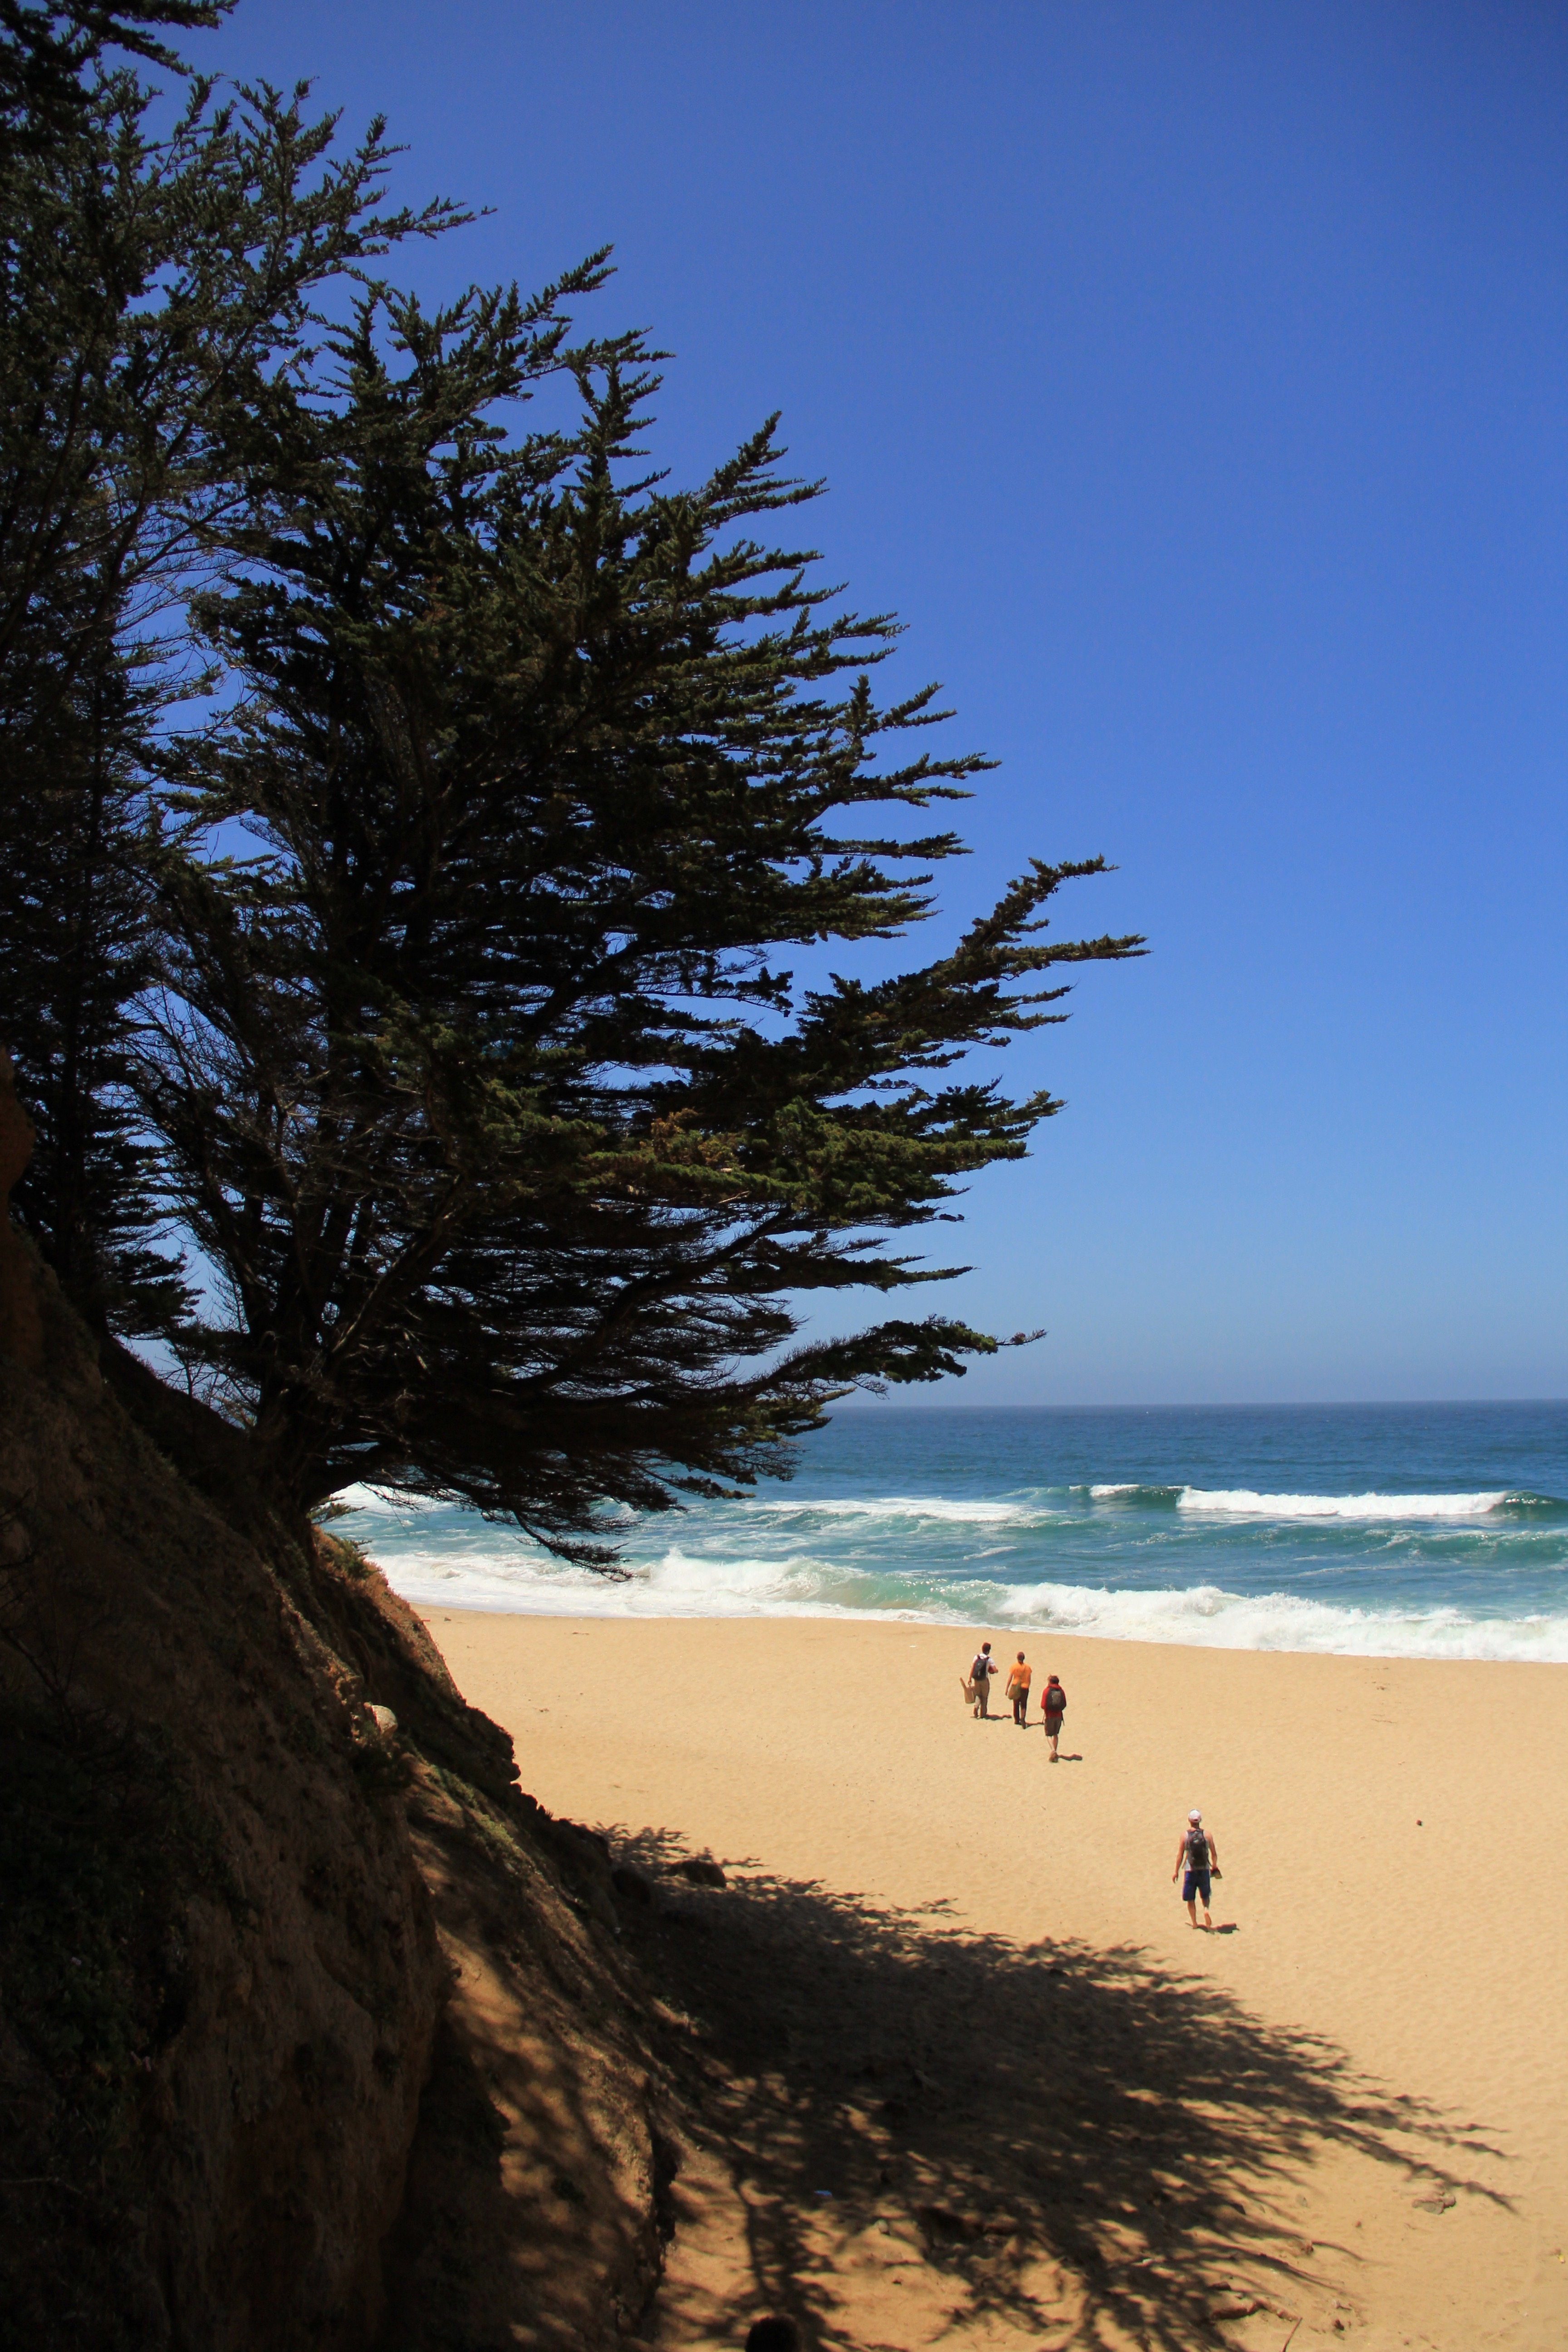
\includegraphics[width = 1.0\paperwidth,
    height = 1.0\paperheight, keepaspectratio]
      {pics/IMG_7946.jpg}}}
        % Adjust filename and path to match your own image 

%%%%%%%Some style changes
\addtolength\textwidth{25mm}
\addtolength\textheight{25mm}
\addtolength\voffset{-5mm}
%\addtolength\oddsidemargin{10mm}
\addtolength\evensidemargin{-20mm}
\usepackage{caption}
\setlength{\captionmargin}{10mm}
\renewcommand\captionfont{\it}
\renewcommand\captionlabelfont{\bf}

\newcommand{\fref}[1]{Figure~\ref{#1}}
\newcommand{\tref}[1]{Table~\ref{#1}}
\newcommand{\tsref}[1]{Tables~\ref{#1}}
\newcommand{\eref}[1]{Equation~\ref{#1}}
\newcommand{\esref}[1]{Equations~\ref{#1}}
\newcommand{\cref}[1]{Chapter~\ref{#1}}
\newcommand{\sref}[1]{Section~\ref{#1}}
\newcommand{\aref}[1]{Appendix~\ref{#1}}
\newcommand{\vecop}[1]{\mathbf{\hat{#1}}}
\newcommand{\op}[1]{\hat{#1}}
\newcommand{\Mu}[0]{\mathrm{Mu}}
\newcommand{\Ref}[0]{\mathrm{ref}}
\newcommand{\tot}[0]{\mathrm{tot}}
\newcommand{\res}[0]{\mathrm{res}}
\newcommand{\In}[0]{\mathrm{in}}
\newcommand{\ud}[0]{\mathrm{ud}}
\newcommand{\out}[0]{\mathrm{out}}
\newcommand{\corr}[0]{\mathrm{corr}}
\newcommand{\quartz}[0]{\mathrm{quartz}}
\newcommand{\fsample}[0]{\mathrm{F}}
\newcommand{\miss}[0]{\mathrm{miss}}
\newcommand{\cor}[0]{\mathrm{cor}}
\newcommand{\cm}[0]{\mathrm{CM}}
\newcommand{\el}[0]{\mathrm{el}}
\newcommand{\mt}[0]{\mathrm{mt}}

%% create blank page
\newcommand{\blankpage}{
\newpage
\thispagestyle{empty}
\mbox{}
\newpage
}

%%%%%%Fliesstext, -bilder
%\usepackage{picins}
%\pichskip{1cm}

\usepackage[hyphens]{url}

%% Define a new 'leo' style for the package that will use a smaller font.
\makeatletter
\def\url@leostyle{%
  \@ifundefined{selectfont}{\def\UrlFont{\sf}}{\def\UrlFont{\small\ttfamily}}}
\makeatother
% Now actually use the newly defined style.
\urlstyle{leo}


%%%%%%Links
\usepackage{color}
\definecolor{DarkBlue}{rgb}{0.1,0,0.55}
\definecolor{olive}{rgb}{0.176,0.498,0.118}
\definecolor{royal}{rgb}{0.412, 0.114, 0.482}
\usepackage[breaklinks=true]{hyperref}
\usepackage[hyphenbreaks]{breakurl}
%%Online version magenta

%%!!!! Important: for the print version, change to black!!!
%\hypersetup{
%   pdfauthor = {author name for pdf},
%	colorlinks=true, citecolor=blue, linkcolor=blue, bookmarksnumbered = true,
 %   }
\hypersetup{
   pdfauthor = {Kim Siang Khaw},
	colorlinks=true, citecolor=blue, linkcolor=blue, bookmarksnumbered = true,
}

%%%%%%Nice Bibliography
%\usepackage[numbers,compress]{natbib} 
\usepackage[numbers,sort&compress]{natbib} 
\usepackage{tocbibind}
\raggedbottom  


%%%%%%Chapter abstract
\newenvironment{chapstract}
{%
\begin{flushright}
\begin{minipage}{0.9\textwidth}
\makebox(0,0)[t]{\hspace*{-1mm}\hspace*{-1mm}\rule{1pt}{15mm}}
\hspace*{-2.5mm}\rule{40mm}{1pt}
\newline
\it
}
{
\end{minipage}
\end{flushright}
\vspace{4mm}
}

%%%%%%Pagestyle

\pagestyle{fancyplain}  
\fancyhf{}  
\renewcommand{\headrulewidth}{0.1pt}  
\addtolength{\headheight}{2.5pt}  
\renewcommand{\chaptermark}[1]{\markboth{#1}{}}  
\renewcommand{\sectionmark}[1]{\markright{\thesection\ #1}}  
\fancyhead[LE]{\textsl{\rightmark}}  
\fancyhead[RO]{\textsl{\leftmark}}  
\renewcommand{\footrulewidth}{0pt}  
\cfoot{\thepage}  

\fancypagestyle{plain}{  
	\fancyhead{}  
	\renewcommand{\headrulewidth}{0pt}  
}  

\renewcommand{\baselinestretch}{1.1}  

\setlength{\parindent}{10pt}

%%%%%%definitions and new commands
%% (just a few examples here)

%openone
\def\openone{\leavevmode\hbox{\small1\kern-3.8pt\normalsize1}}%
%Spinor
\newenvironment{spinor}
{%
\left\{\!\!
\begin{array}{c}
}
{
\!\!
\end{array}
\!\!\right\}
}

%ETHFont fuer Titelseite / for frontmatter
\renewcommand{\sfdefault}{let}

% Acronyms
\usepackage[printonlyused]{acronym}

% Additional operators used
\DeclareMathOperator{\tr}{Sp}
\DeclareMathOperator{\im}{Im}

% Hamiltonian
\newcommand{\HH}{\mathcal{H}}

% vectors
%\newcommand{\vr}[1]{\mathbf{#1}}
\newcommand{\vr}[1]{\boldsymbol{#1}}

